\newpage
\section{Klassifikation}\label{kap:klassifikation}
In Kapitel \ref{kap:detektion} wurde beschrieben, wie die Positionen aller Kugeln mithilfe eines Bilds des Spielstands detektiert werden.
Um den Spielstand zu verstehen ist es relevant zu wissen, welche Kugel welche Farbe hat.
Im Snooker gibt es die Farben Weiss, Rot, Gelb, Pink, Grün, Blau, Braun und Schwarz.
Deshalb muss jede detektierte Kugel anhand eines Bildausschnitts in eine dieser Klassen eingeteilt werden.
Der Ablauf der Klassifikation der Snooker-Kugeln wird nachfolgend beschrieben.

Zunächst liegt zu jeder Kugel deren Position in Pixel- sowie Modell-Koordinaten vor und der Radius der Kugeln ist in Pixel bekannt\cite{project2:pixel_to_model_coordinates}.
Aufgrund dieser Informationen wird von jeder detektierten Kugel ein Bildausschnitt des RGB-Bildes rund um die Kugelposition definiert,
der für die Klassifikation verwendet werden kann.
Der Bildausschnitt ist quadratisch, wodurch in den Ecken des Bildes noch das Grün des Billardtisches ersichtlich ist.
Dieses Grün könnte die Klassifikation verfälschen, da damit mehr grüne Pixel auf dem Bild sind und eine Kugel eher als grün klassifiziert werden könnte.
Um dieses Problem zu umgehen wird der Pixelradius der Kugel mit einem Faktor von $0.5$ skaliert, um den Bildausschnitt zu verkleinern
und den grünen Tisch so zu entfernen, siehe Abbildung \ref{fig:klassifikation_radius}.

\begin{figure}[h!]
    \centering
    \begin{subfigure}[t]{0.3\textwidth}
        \centering
        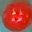
\includegraphics[width=1.0\linewidth]{../common/03_billiard_ai/resources/classification/radius_full.png}
        \caption{
            Quadratischer Bildausschnitt einer Kugel mithilfe des berechneten Radius einer Kugel in Pixel.
            In den Ecken ist das Grün des Billardtisches sichtbar, welches die Klassifikation verfälschen könnte.
        }
        \label{fig:klassifikation_radius_full}
    \end{subfigure}
    \begin{subfigure}[t]{0.3\textwidth}
        \centering
        
\includegraphics[width=1.0\linewidth]{../common/03_billiard_ai/resources/classification/radius_reduced.png}
        \caption{
            Verkleinerter Bildausschnitt derselben Kugel wie in Abbildung \ref{fig:klassifikation_radius_full},
            bei dem das Grün des Billardtisches nicht mehr sichtbar ist.
        }
        \label{fig:klassifikation_radius_reduced}
    \end{subfigure}
    \caption{Auswahl aus den Trainingsbilder}
    \label{fig:klassifikation_radius}
\end{figure}

Für die Entwicklung der Klassifikation wurden einige Trainingsbilder von verschiedenen Spielständen gemacht,
anhand derer die Parameter eingestellt wurden.
In diesen Trainingsbildern ist eine Kugel jeder Klasse an unterschiedlichen Stellen platziert worden,
um die ungleichmässige Ausleuchtung des Billardtischs zu berücksichtigen.
In Abbildung \ref{fig:classification_trainingdata_examples} sind zwei Trainingsbilder pro Klasse aufgeführt.

\begin{figure}[h!]
    \centering
    \begin{subfigure}[b]{0.15\textwidth}
        \centering
        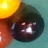
\includegraphics[width=1.0\linewidth]{../common/03_billiard_ai/resources/classification/BLACK_1.png}
        \caption{Schwarz 1}
        \label{fig:classification_black_ball_1}
    \end{subfigure}
    \hfill
    \begin{subfigure}[b]{0.15\textwidth}
        \centering
        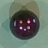
\includegraphics[width=1.0\linewidth]{../common/03_billiard_ai/resources/classification/BLACK_2.png}
        \caption{Schwarz 2}
        \label{fig:classification_black_ball_2}
    \end{subfigure}
    \hfill
    \begin{subfigure}[b]{0.15\textwidth}
        \centering
        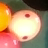
\includegraphics[width=1.0\linewidth]{../common/03_billiard_ai/resources/classification/WHITE_1.png}
        \caption{Weiss 1}
        \label{fig:classification_white_ball_1}
    \end{subfigure}
    \hfill
    \begin{subfigure}[b]{0.15\textwidth}
        \centering
        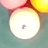
\includegraphics[width=1.0\linewidth]{../common/03_billiard_ai/resources/classification/WHITE_2.png}
        \caption{Weiss 2}
        \label{fig:classification_white_ball_2}
    \end{subfigure}
    \hfill
    \begin{subfigure}[b]{0.15\textwidth}
        \centering
        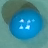
\includegraphics[width=1.0\linewidth]{../common/03_billiard_ai/resources/classification/BLUE_1.png}
        \caption{Blau 1}
        \label{fig:classification_blue_ball_1}
    \end{subfigure}
    \hfill
    \begin{subfigure}[b]{0.15\textwidth}
        \centering
        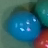
\includegraphics[width=1.0\linewidth]{../common/03_billiard_ai/resources/classification/BLUE_2.png}
        \caption{Blau 2}
        \label{fig:classification_blue_ball_2}
    \end{subfigure}
    \hfill
    \begin{subfigure}[b]{0.15\textwidth}
        \centering
        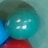
\includegraphics[width=1.0\linewidth]{../common/03_billiard_ai/resources/classification/GREEN_1.png}
        \caption{Grün 1}
        \label{fig:classification_green_ball_1}
    \end{subfigure}
    \hfill
    \begin{subfigure}[b]{0.15\textwidth}
        \centering
        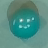
\includegraphics[width=1.0\linewidth]{../common/03_billiard_ai/resources/classification/GREEN_2.png}
        \caption{Grün 2}
        \label{fig:classification_green_ball_2}
    \end{subfigure}
    \hfill
    \begin{subfigure}[b]{0.15\textwidth}
        \centering
        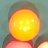
\includegraphics[width=1.0\linewidth]{../common/03_billiard_ai/resources/classification/YELLOW_1.png}
        \caption{Gelb 1}
        \label{fig:classification_yellow_ball_1}
    \end{subfigure}
    \hfill
    \begin{subfigure}[b]{0.15\textwidth}
        \centering
        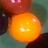
\includegraphics[width=1.0\linewidth]{../common/03_billiard_ai/resources/classification/YELLOW_2.png}
        \caption{Gelb 2}
        \label{fig:classification_yellow_ball_2}
    \end{subfigure}
    \hfill
    \begin{subfigure}[b]{0.15\textwidth}
        \centering
        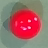
\includegraphics[width=1.0\linewidth]{../common/03_billiard_ai/resources/classification/RED_1.png}
        \caption{Rot 1}
        \label{fig:classification_red_ball_1}
    \end{subfigure}
    \hfill
    \begin{subfigure}[b]{0.15\textwidth}
        \centering
        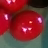
\includegraphics[width=1.0\linewidth]{../common/03_billiard_ai/resources/classification/RED_2.png}
        \caption{Rot 2}
        \label{fig:classification_red_ball_2}
    \end{subfigure}
    \hfill
    \begin{subfigure}[b]{0.15\textwidth}
        \centering
        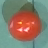
\includegraphics[width=1.0\linewidth]{../common/03_billiard_ai/resources/classification/BROWN_1.png}
        \caption{Braun 1}
        \label{fig:classification_brown_ball_1}
    \end{subfigure}
    \hfill
    \begin{subfigure}[b]{0.15\textwidth}
        \centering
        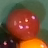
\includegraphics[width=1.0\linewidth]{../common/03_billiard_ai/resources/classification/BROWN_2.png}
        \caption{Braun 2}
        \label{fig:classification_brown_ball_2}
    \end{subfigure}
    \hfill
    \begin{subfigure}[b]{0.15\textwidth}
        \centering
        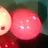
\includegraphics[width=1.0\linewidth]{../common/03_billiard_ai/resources/classification/PINK_1.png}
        \caption{Pink 1}
        \label{fig:classification_pink_ball_1}
    \end{subfigure}
    \hfill
    \begin{subfigure}[b]{0.15\textwidth}
        \raggedright
        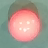
\includegraphics[width=1.0\linewidth]{../common/03_billiard_ai/resources/classification/PINK_2.png}
        \caption{Pink 2}
        \label{fig:classification_pink_ball_2}
    \end{subfigure}
    \caption{Auswahl aus den Trainingsbilder}
    \label{fig:classification_trainingdata_examples}
\end{figure}

Eine Klassifikation dieser Kugelfarben findet sinnvollerweise nicht im RGB-Farbraum, sondern im HSV-Farbraum\cite{wiki:hsv_color_space} statt.
Dadurch gehören beispielsweise die roten, pinken und braunen Kugeln in den roten Bereich des Hue-Kanals.
Die weisse und die schwarze Kugel sind am ehesten im Value-Kanal klassifizierbar.

Zunächst wird zur Rauschunterdrückung ein Gauss-Filter mit der Kernelgrösse von 5x5 auf den zu klassifizierenden Bildausschnitt angewendet.
Anschliessend wird das RGB-Bild in den HSV-Farbraum konvertiert, um die Farbanalyse zu vereinfachen.
Aufgrund des HSV-Bildes wird pro Kanal (Hue, Saturation und Value) ein Histogramm berechnet und der häufigste Wert ermittelt.
Damit wurde die Information des Bildausschnitts auf drei Zahlen, eine pro HSV-Kanal, reduziert.
Diese drei Werte können als Position des Bildausschnitts im HSV-Raum interpretiert werden.

In Abbildung \ref{fig:klassifikation_cluster} ist der HSV-Farbraum der Trainingsbilder abgebildet.
Für jedes Trainingsbild wurde die zuvor erklärte Position im HSV-Raum eingezeichnet.
Aus diesem Clusterdiagramm können einige Schlüsse gezogen werden.
Die Klassifikation der blauen und grünen Kugeln erdordert lediglich den Hue-Kanal (oben-links).
Die schwarze Kugel kann über den Value-Kanal (unten-rechts) klassifiziert werden.
Die roten und braunen Kugeln liegen dicht beieinander, wobei die Sättigung (mitte-rechts oder unten-mitte) ein gewisses Unterscheidungskriterium bildet.

\begin{figure}[h!]
    \begin{center}
        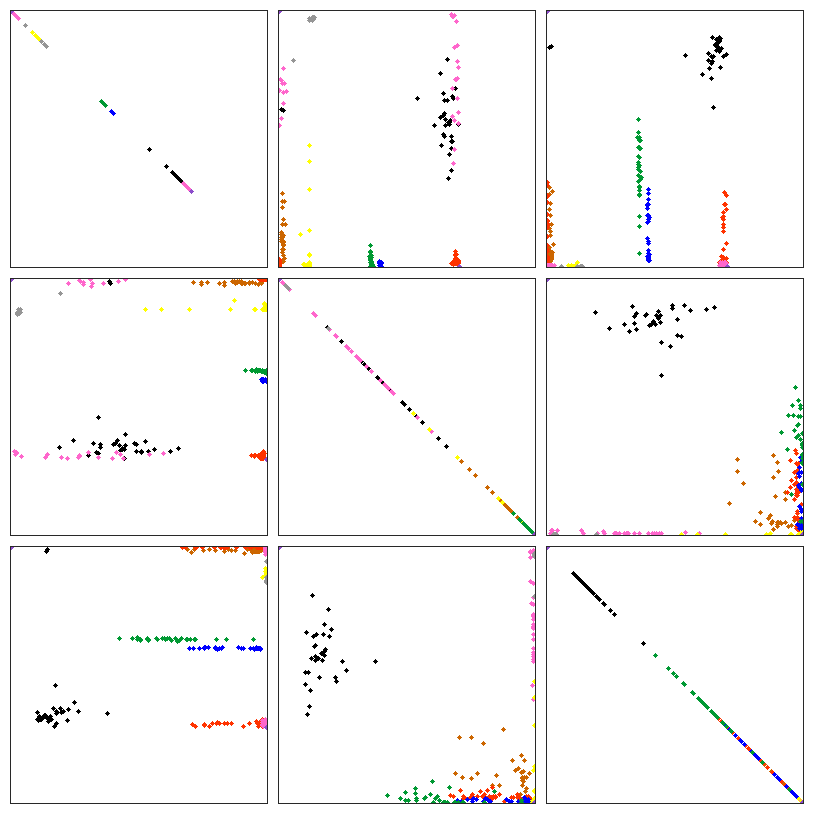
\includegraphics[width=0.7\linewidth]{../common/03_billiard_ai/resources/classification/Cluster_all.png}
    \end{center}
    \caption{
        Paarweise Gegenüberstellung von HSV-Kanälen mit eingezeichneten Datenpunkten der Testbilder.
        Vertikal sind von oben nach unten die Kanäle Hue, Saturation und Value abgebildet.
        Horizontal sind von links nach rechts die Kanäle Hue, Saturation und Value abgebildet.
        Die Farbe der Datenpunkte entspricht ihrer Klasse, wobei die Klasse \emph{weiss} mit grauer Farbe gezeichnet wurde.
        Es ist zu beachten, dass der Hue-Kanal hierbei einen Wertebereich von [0, 180] hat, währenddessen
        der Saturation- und Value-Kanal einen Wertebereich von [0, 255] aufweisen.
    }
    \label{fig:klassifikation_cluster}
\end{figure}

Das Resultat der Analyse dieser Daten sind Wertebereiche für die HSV-Kanäle pro Klasse, wodurch eine grobe Klassifikation,
ermöglicht wird.
Diese Wertebereiche bieten keine eindeutige Klassifikation, sondern werden verwendet, um die potenziellen
Klassen einer Kugel zu finden.
So kann es sein, dass eine blaue Kugel aufgrund ihres Hue-Kanals klar als Blau erkannt wird.
Es kann aber auch sein, dass eine braune Kugel sowohl Rot, Pink und Braun als potenzielle Klassen erhält.

Es muss demnach noch eine genauere Unterscheidung gemacht werden, sobald die potenziellen Klassen bekannt sind.
Anhand der Trainingsbildern wurden die Durchschnittswerte der häufigsten Werte der HSV-Kanäle pro Klasse berechnet.
Diese Durchschnittswerte bilden die Cluster-Zentren jeder Klasse und können für die Klassifikation verwendet werden.
Dazu wird die Distanz der HSV-Position des zu klassifizierenden Bildausschnitts zu jedem Cluster-Zentrum bestimmt.
Der Cluster mit der kleinsten Distanz gibt dem Bildausschnitt seine Klasse.

Sofern ein Bildausschnitt mehrere potenzielle Klassen in der Prüfung durch Wertebereiche erhalten hat, wird die Distanz
zwischen dessen HSV-Position und dem Cluster-Zentrum jeder der potenziellen Klassen verglichen.
Die Klasse mit der kleinsten Distanz zur HSV-Position des Bildausschnitts wird angenommen.
Demnach ist diese Klassifikation in der Idee ein \emph{k-nearest neighbors} Algorithmus\cite{wiki:k_nearest_neighbors},
wobei keine Trainingsdatensätze als Nachbaren verwendet werden, sondern die bereits gefundenen Cluster-Zentren.

Sofern ein Bildausschnitt keine potenziellen Klassen erhalten hat, wird diesem die Klasse \emph{unbekannt} zugewiesen.

Mit der hier beschriebenen Klassifikation ist die Farbe jeder Kugel nach deren Detektion bekannt und es
sind alle Informationen für die weitere Verwendung in der Suche und Darstellung vorhanden.
